
% \title{The Statistical Analysis of Electoral Alliances}



% \author{Eduardo L. Leoni \\Department of Political Science\\
% Columbia University   \\
% 7th Floor, International Affairs Bldg. \\
% 420 W. 118th Street \\
% New York, NY 10027 \\
% %% Mail Code 3320 \\
% email: ell2002@columbia.edu}
% \date{}

% \maketitle \thispagestyle{empty}
% \bigskip
% \bigskip

% \abstract{In this paper we derive a statistical model from  an expected utility theory of electoral coalition formation in proportional representation systems. The theory predicts that parties are more likely to form a coalition if they are ideologically closer to each other. In addition, there is a party specific threshold that tells us how far the other party can be located and still asked to form a coalition. This threshold depends on the share of votes the party is expected to get and the magnitude of the district.  The statistical model we derive  is able to simultaneously estimate the ideological position of parties and the structural parameters relating  district magnitude and party size to coalition formation. We apply the model to the Brazilian local legislative elections of 2000 and find broad support for our hypotheses. Ideological distance, district magnitude and party vote-shares have negative effects on the likelihood of coalition formation. Moreover, the mean party locations derived from the model are highly correlated with the party locations estimated using roll call data in the national legislature. We also present arguably the first estimates of state-level positions of Brazilian political parties, and find that they are broadly consistent with hypotheses gathered from the Brazilian politics literature.}

% \end{titlepage}


%%TO DO
%% How is the number of seats decided?



%%Graham p.148 First, citizens divided politically not because of party loyalties, much less ideological considerations, but because of personal ties, making party labels seriously misleading at both the local and the national level. Second, power flowed simultaneously ``downwards'' from the Cabinet through the provincial president and ``upward'' from local bigwigs to the president and Cabinet in eddies and swirls that defy simple summary.

%\doublespace
%POOLE
%(1) a deterministic component that is a function of the distance between the 
%legislator and a roll call outcome; and (2) a stochastic component that represents the 
%idiosyncratic component of utility.
%Jackman on gelman's blog http://www.stat.columbia.edu/~cook/movabletype/archives/2004/11/ideal-point-mod.html
% One of the things I like about the setup in my work with Doug & Josh is that (1) our statistical model falls out of a fairly standard formal-theoretic approach to roll call voting (the Euclidean spatial voting model with quadratic utilities over outcomes and local/conditional independence); (2) our setup maps directly onto the 2 parameter IRT model from educational testing, about which much is known... In this sense our approach is a little more model-driven than data-driven (i.e., contrast naive MDS or factor analysis or clustering etc). My experience is that anything too data-driven in this field tends to run into trouble within political science because it while it is one thing to toss more elaborate statistical setups at the roll call data, they tend to lack the clear theoretical underpinnings of the Euclidean spatial voting model. Put differently, what is the model of legislative decision-making that underpins any given statistical model?

% What behavioral/political assumptions or processes suggest that we ought to do this when we model the data? The point here is that things that sometimes make good sense or seem attractive from a statistical perspective will often into a wall of skepticism from Congress people who like to see things built up from ground zero (legislators' utility functions...). 

%Gelman : I agree with you completely on the desirability of an individual-level "agent" model, which ideally (as in your work) can imply a statistical model.

% \begin{quote}
%   A coalitional structure is a partitioning of the set of players into a collection of groups, 􏰂 = (G j ) m j =1 , such that everybody is in some group ( ∪ m j =1 G j = N ) and no one is in two groups (G j ∩ Gk = ∅ for j ̸= k). Typically, we assume that a parti- tioning is defined uniquely up to the reordering of cells and of individuals within cells (thus {{1,2},{3,4}} is considered the same partition as {{4,3},{1,2}}). Let the set of all such parti- tions be given by G . For a population of size n, the cardinality of G is then given by the Bell number (Rota 1964), a number that grows very rapidly in n. The set of partitions for n = 4 is 15. For a 100-person senate, the Bell number is on the order of 10116 (Weisstein 2005).
% \end{quote} \citep{humphreys:2008}

% \begin{itemize}
% \item Parties decide, not ``coalitions''
% \item Spatial distance + valence matter
% \item Simplify the partition problem into binary decisions
% \item Formalize what assumptions are being made
% \end{itemize}

% For concreteness, let's assume there are three parties in the polity. We are interested on the parties' decisions to form electoral coalitions. 

% The possible partitions with three parties are:

% \begin{verbatim}
% {a,a,a} (A coalition of all parties)
% {a,b,a} (Parties 1 and 3 join a coalition a. Party 2 competes alone.)
% {a,a,b}
% {b,a,a}
% {a,b,c} (Each party competing separately)
% \end{verbatim}

% We are interested in casting the decision of which coalition structure to form in terms of each of the individual parties' decision to join a specific coalition. Note, in addition, that one can observe only one of those coalitional structures at each coalition opportunity for the parties. The number of possible coalitional structures, or set partitions, possible  is given by the Bell number $B(n)$\citep{rota:1964}. This number will grow very fast. With four parties, the number of possible partitions is 15; with seven (the number of effective parties in Brazil) it is 877. With 10 parties (half the number of parties represented in the Brazilian lower chamber) the Bell number is  115975. Without further simplifications it is  extremely difficult analyze all coalition decisions when the number of parties is moderate to large as in the Brazilian case.

% Therefore, we should look into ways to simplify the individual parties decisions. First, given that a particular coalition forms, what must be true about the utilities of the parties involved? This depends on the utility functions of the parties and on the particular game being played by the parties when forming coalitions.

% I illustrate the bias in traditional methods and apply a permutation test to one practical 
% example. Scholars in recent years have used group vs. subgroup comparisons to explore the 
% impact of federal forms of government on legislative party systems. The basic arguments are 
% as follows. Federal forms of government create and/or strengthen state-level (or province- 
% level) interests. Legislators in many national Congresses are accountable to state-level actors 
% for nomination, election, or career advancement. Consequently, national parties may split 
% on questions that mobilize pressure or that greatly affect state interests. To the extent that 
% these forces are at work, national-party cohesion should be lower because of the federal 
% form of government. 
% One country where this argument has been applied is Brazil. A federal republic with 
% 26 states and a federal district, Brazilian state politics have been characterized as having 
% important national effects. Brazilian federalism places key political resources in the hands of 
% state actors, granting them influence over the behavior of national legislators and weakening 
% national-party leaders (Mainwaring 1997, 1999; Selcher 1998; Souza 1998; Ames 2001; 
% Samuels 2002). For example, initial nominations to run for Congress and access to free 
% media time for campaign advertisements are both controlled by state parties. Similarly, state 
% governors distribute many political jobs, including coveted directorships of state agencies. 
% Consequently, “Politicians of the catchall parties focus a lot on state and local issues, so they 
% are less likely to toe the line of the national party leadership” (Mainwaring 1997, p. 83). As 
% a result, “. . .[f]ederalism influences the party system because most key decisions are made 
% at the state level and abundant resources are allocated at this level” (Mainwaring 1999, 
% p. 263). 


% These numbers, large as they seem, pale when confronted to what could have happened. There are more than two billion possible coalitions with two or more parties that can form in a party system with 31 parties. The number of possible ways to arrange these parties into electoral coalitions is orders of magnitude larger.\footnote{The number of possible partitions of a set of size $N$ is the Bell number of $N$\citep{rota:1964}.} Even if we concentrate on the 8 largest parties in Brazil, there are more than four thousand different coalitional structures that can emerge in each of the 5559 local elections in 2000. In this paper, we argue that a well grounded theoretical model can help simplify the statistical analysis while aiding in the interpretation of the results. %The main output of our model are estimates of the ideological positions of parties in each of the 26 Brazilian states.

% \begin{quote}
% In contrast, the spatial theory of voting is a \emph{theory of behavior}  that states that \emph{if} a set of assumptions holds, \emph{then}  voters should behave ina certain way \emph{and} we should observe certain types of outcomes. It is a theory that makes predictions that can be tested.\citep[p.9]{poole:2005}
% \end{quote} 

% \begin{quote}
%   Brazil has long been the case of most robust federalism in Latin America \dots By robust federalism, I mean that, during democratic periods, mayors and governors have been powerful actors with significant autonomy vis-à-vis the federal government and with significant resources. The catchall parties are decentralized, and parties and politicians generally follow a logic of federalism. Many of their actions are determined more by what goes on in their own states than by what goes on in national politics. In fact, the national parties are still to a considerable extent a federation of state parties.\citep[p.83]{mainwaring:1997a}\end{quote} 


% * Why do parties form coalition in advance of elections?
% * Coalition formation as surplus of votes sharing.

%\singlespace
\epi{Brazil is very uneven,  just a mess. One cannot understand it.}{Federal deputy and mayor Luciano Castro (PR-RR), commenting on the different political alliances at the national and local levels in Brazil. \\ Folha de São Paulo, June 29th \citeyear{bragon:2008}.}

\epi{(C)itizens (are) divided politically not because of party loyalties, much less ideological considerations, but because of personal ties, making party labels seriously misleading at both the local and the national level. }{\citet[p.148]{graham:1990} on political parties in 19th century Brazil.}
%\doublespace


Why do parties form coalitions?  Research into this question in comparative politics has mainly focused on the formation of \emph{government} coalitions in  parliamentary systems \citep{martin:2001a} and coalition support for the president in separation-of-powers systems  \citep{neto:2006,altman:2000}.  More recently, some attention has been paid to the electoral coalition agreements among parties in parliamentary systems \citep{blais:2008,golder:2006a}. 

In this paper, we focus on the electoral alliance decisions in local legislative elections in Brazil. Building on pioneering work by \cite{soares:1964}, the alliance formation theory we propose has the following characteristics. We assume that parties  have ideal points in a one-dimensional policy space. When forming alliances, parties want to maximize the number of seats won in the election while minimizing the ideological distance between the alliance members' ideal points. The incentives for alliance formation depend, then, on the ideological preferences of the potential alliance partners and the constraints imposed by political  (the expected party share of the votes) and institutional (the magnitude of the district) context. We derive a statistical model from these assumptions, which allows us to estimate both the spatial location of parties and the structural parameters of the model.

The statistical model we propose is closely related to ideal point estimation methods that rely on roll call data. Such models require  repeated decisions by the same actors in a large number of elections. The massive data available from the Brazilian local legislative elections provide us an excellent opportunity to estimate models of electoral alliance formation. In the elections of 2000, 368 thousand  candidates competed  for the  60 thousand  municipal legislators seats available in the more than five thousand independent elections (one per municipality) across the nation. The number of seats in each election varied from 9 (the constitutionally mandated minimum) to 55.  The number of candidates in each election ranged from 9 (in São Julião, Piauí state) to 1095 (in São Paulo, São Paulo state).  Candidates competed as members of 31 political parties under open-list proportional representation using the D'Hondt method. Parties were free to form  pre-electoral alliances (\emph{coligações}) in each election. There were 2845 different electoral alliances formed in the 2000 elections.

Since local political institutions in Brazil follow a separation-of-powers structure, we argue that these alliances do not form in order to attain a majority in the legislature. These pacts, after all,  are frequently different from those agreed upon for the competition for the Mayoral offices that occur simultaneously with the local legislative elections.  We argue instead that electoral alliances are simply pre-electoral agreements to share surplus votes when translating votes to seats. 

We find that there is an important ideological component to the parties' decisions to form pre-electoral alliances. Alliances more frequently arise between parties that are closer to each other in the ideological space. The overall party ordering estimated using the alliance data is highly correlated with the positions estimated using roll calls in the national legislature, giving some face validity to the model.  We also find that the institutional and political contexts, specifically the district magnitude and the size of the political party in the district, are just as important to the alliance decisions. 

The paper is structured as follows. First we outline the institutional features of local legislative elections in Brazil and briefly summarize the literature on this question. We then discuss the problems  of measuring ideology in Brazil and argue that the alliance data is a potentially good source for estimating party ideal points. Next, we present our statistical model of alliance formation and show the results from estimating our model using the 2000 elections. We  conclude by discussing possible  extensions to our model and its applicability in other contexts.

\section{Electoral alliances in Brazil}
\label{sec:measuring-ideology}


In the 2008 election for mayor in the Brazilian fourth largest city, Belo Horizonte, the two main opposing parties in Brazil -- PT (Workers Party) and PSDB (Social Democratic Party) -- formed an (informal) alliance.  If one looks at roll calls in Congress, these parties couldn't be farther apart \citep{leoni:2002}. Yet, an alliance between the state governor (Aécio Neves, PSDB) and the then mayor\footnote{Executive political positions in Brazil (mayors, governors and Presidents) can only be re-elected once.} (Fernando Pimentel, PT) was formed to (successfully) elect Márcio Lacerda (PSB) as mayor. 

The dissonance between local and national politics is seemingly maddening even for professional politicians and academics. In this paper, however, we show that there is an ideological structure in the electoral alliance decisions in local legislative elections in Brazil.  The theory we propose is simple, taking into account electoral imperatives and ideological preferences. In addition, since these decisions are made by the rank-and-file of the political parties, this analysis of alliance decisions serves to illuminate the interplay of politics at the national and regional levels. 

Local legislators in Brazil are elected under open-list proportional representation using a modified D'Hondt system. In this system,  voters  cast their vote for a specific candidate or for a political party. Votes are then aggregated up to the electoral list. The D'Hondt formula is used to distribute seats to lists, while  candidates within each list are ordered according to how many individual votes they received in the election.  The only modification to the D'Hondt system is that parties/alliances that received less than one ``electoral quotient'' (sum of valid votes divided by the number of seats) do not receive any seats. This means that there is an effective threshold of 1/number of seats, ranging from 11 \% in the smallest cities to 2\% in the largest city. This provides a substantive incentive for small parties to form alliances in small cities. 

The mechanical effect of the modified D'Hondt system on total party shares of local legislators in Brazil is plotted n Figure \ref{fig:comp}.  Only the three largest parties in Brazil (PSDB, PMDB and PFL) are net winners of seats if seat assignments where calculated without electoral alliances.   

 \begin{figure}
  \centering
  \includegraphics[width=.5\textwidth]{/Users/eduardo/reps/Brazilian-Local-Elections/results/Vereador/2000/comparisonPoints.pdf}
  \caption{The percent of votes for parties in Brazil in the 2000 elections summed over all municipalities plotted against .  }
  \label{fig:comp}
\end{figure}


% There are N votes in an election to select M legislators. 
Invalid votes and abstentions are excluded from the calculations. Votes are cast for individual candidates or parties, but  87\% of the voters select a specific candidate. All votes are aggregated up to electoral lists. Electoral lists may be made up by more than one party, joined together in an electoral alliance (\emph{coligação}). Fundamentally, an electoral alliance is an agreement to share ``surplus'' votes across political parties. Perhaps as importantly in the largest municipalities, parties also agree to share the assigned free television time they have. Elections for mayors and local legislators are held concurrently in the midterm of the national elections.

That parties and alliances play a minor role in elections in Brazil can be glanced from political advertisement in Brazil.  Figure \ref{fig:add_sp} shows a typical political advertisement that can be found in the Brazilian streets during election season. The add is dominated by the face,   name and number of the candidate. The number is important, since knowing it is necessary for the voter to cast his/her vote to a specific candidate in the voting booth. Brazil uses electronic voting since the 1996 elections. The party of the candidate occupies a very small space in the add. Finally, there is usually some reference to the candidate of the Executive post (Mayor, in this case). 

\begin{figure}
  \centering
  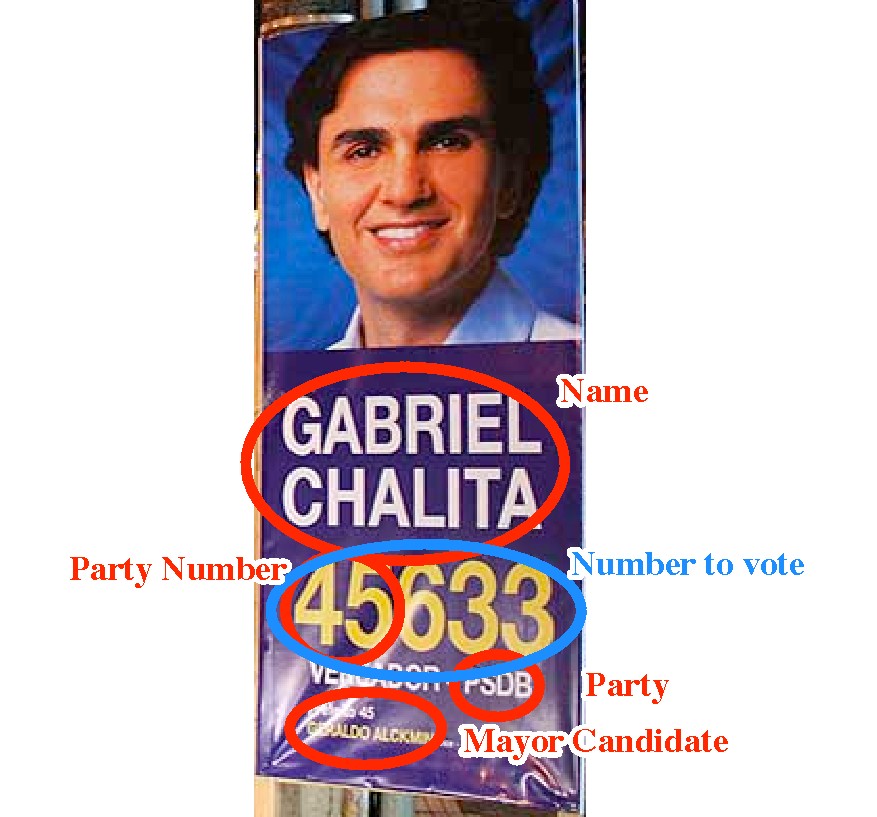
\includegraphics[width=.5\textwidth]{../images/alliances/propaganda_sp.pdf}
  \caption{Add for a Vereador candidate in São Paulo. Note that the picture of the candidate covers most of the add and the party label is comparably very small. The alliance is nowhere to be seen.}
  \label{fig:add_sp}
\end{figure}


There is a growing literature on the analysis of electoral alliances in Brazil. The pioneering work was done by  \citet{soares:1964}. Making use of the \citet{downs:1957}'s spatial theory of democracy, Soares proposed two theories/hypotheses to account for electoral alliance formation in Brazil.  The  ``cost minimization theory'' hypothesis  states that parties will form alliances 
in order to maximize their seat shares given the number of votes they expect to get in the forthcoming elections. The ``ideological resistance'' hypothesis states that parties prefer to form alliances with parties that have similar ideological positions. 

That article ignited a cottage industry of papers studying electoral alliances in Brazil, which has been particularly active in the recent period.\footnote{\citet{miguel:2007} provide an excellent review of the literature.} This literature, however, faces a couple of serious short-comings. First, the ideology measures used are hard to replicate and not explicitly linked to any sort of political behavior. Secondly, the theoretical development seem to have stagnated with Soares article from four decades ago. ``Ideological resistance'' and ``cost minimization'' are seen as ``either-or'' propositions, without an integrated way to think about how they both might affect party behavior. A final problem is the lack of a statistical model, without which the  importance of ideology and/or  ``cost minimization'' hypotheses on party behavior cannot be ascertained. 






\section{On   ideology and its measurement}

Ideology in modern political science is currently thought as a theory of political behavior. We  start by assuming that the policy space is high dimensional. For instance, views about international trade, government support for child care, abortion, taxes, etc, can all vary independently across voters and politicians. However, research  has shown that most of the issues governing the day are highly correlated, so that when one analyzes the actions of decision makers, just one or two dimensions might be sufficient to explain most of the behavior. This low dimensional space is called ``predictive'', ``basic'' \citep[p.13-14]{poole:2005} or, most commonly, ``ideological'' space \citep{hinich:1994}.   

If we define ideological space as the predictive dimensions of political behavior, it is not surprising to note that state of the art measurement models of ideology derive ideal point estimates from observed political action. There is a long and noble tradition of measuring  ideology of legislators using their roll call votes.\citep[e.g.]{poole:1997}. \citet[p.355]{clinton:2004} go so far as stating that the ``primary use of roll call data is the estimation of ideal points.''  As these authors note, roll calls are effective measures for  describing  the behavior of legislators. There are a many other things that legislators do, of course. But roll calls are both readily available in many legislatures, and also important since they record preferences over actual policies. Researchers also use roll calls in order to \emph{test} spatial theories of political behavior.  In this tradition, one starts by formulating a (formal) theory of behavior, derives the implications of such theory and then estimates a model that follows from it.\cite[p.9]{poole:2005} 

One should note that there is nothing particularly special about roll call data: any other record of behavior that can be thought of as a consequence of the theory being tested is likely to be just as useful. What is in fact special about roll call data is the extraordinary quantity and time-span of such data  for the United States Congress and many other legislatures across the world.

% There is a well known problem with roll call data, however. If, for example, the agenda is controlled by the majority party leadership, bills that would divide the majority party are not likely to reach the floor. 

In Brazil a one dimensional model of roll call behavior seems  to fit well the data \citep{leoni:2002}.  The two-dimensional ideal points  for legislators in the legislative sessions from 1991 until 2006 are displayed in Figure \ref{fig:wnominate}, along with estimated cutting-lines\footnote{We used the \texttt{wnominate} \citeyear{poole:2007} \texttt{R} package to perform estimation and plots.} . The cutting-lines are estimates of the lines separating legislators voting \emph{Yea} from those voting \emph{Nay}.  A one dimensional model predicts correctly around 88\% of the roll call votes in the 1991-1996 session and 92\% in the legislative sessions from 1995 until 2006. 

\begin{figure}
  \centering
  \includegraphics[width=.9\textwidth]{/Users/eduardo/projects/BrazilianPolitics/trunk/dissertation/hip/wnominate_plot.pdf}
  \caption{\textsc{W-NOMINATE} ideal point estimates of the Brazilian Chamber of Deputies, 1991-2006. Note how, starting in the 1995-1998 session, cutting lines are almost all vertical and concentrated in a small portion of the state.}
  \label{fig:wnominate}
\end{figure}

The Figure is interesting for what it does \emph{not} show: from 1995 to 2002 the roll call cutting-lines almost never separate parties in the majority. The majority is located in the right side of the space in the 1991-2002 sessions and in the left side of the space in the 2003-2006 session.   Since roll calls do not split the majority parties, there is limited information available in them that is useful to differentiate parties \emph{within} the majority.

Another, more serious, problem is that the estimated ideal points can only be treated as such (ideological ideal points) if  roll call behavior is driven predominantly by spatial preferences. Let $i$ index legislators and $j$ index roll calls. A function linking preferences $x_i$ to roll call behavior $y_{ij}$ can be written as:

\begin{equation}
  \label{eq:3}
  y_{ij} = f(\alpha_j+x_i\beta_j +e_{ij})
\end{equation}

That is, the model assumes that only preferences drive behavior. More precisely, the errors $e_{ij}$ are independent and identically distributed. If, however, there is some sort of vote buying $z_{ij}$ that is not constant across legislators, then estimated ideal points will be biased. This would be of not much consequence if all we want is a description of roll call behavior, but insufficient if we want to test a theory of behavior. In the case of Brazil, part of the literature claims there is a \emph{quid pro quo} between Presidents and legislators.\citep{alston:2006,alston:2007,zucco:2007} Presidents  have the authority to withhold expenditures under the Brazilian Constitution, so, according to the argument in these articles, they have leverage when dealing with legislators.  Since such vote buying is in general inconsistent with pure spatial voting, the usual estimators of ideal points will lead to misleading estimates of preferences. This argument is more fully developed by \citet{zucco:2009}. He combines roll call data with a self-positioning of legislators measured using surveys and finds that the influence of ideology (as measured by the surveys) on roll call behavior of deputies has declined over time in Brazil. 

Another way to deal with the issue is to find data where such constraints (e.g. vote buying) are not as relevant. \citet{groseclose:2000}  argue that measuring ideology lop-sided roll calls in Congress are closer to the ``true'' preferences of legislators, and the difference between these preferences measured using lop-sided votes and preferences measured using non lop-sided serve as a measure of party influence on roll call behavior. More generally, we want to find behavior that is important  (behavior that ``matters'') but not overwhelmingly influenced by outside actors (e.g. the President).  In this vein,  \citet{monroe:2008} propose to measure ideal points using political text and speech; \citet{aleman:2009} use cosponsorship, that is, data on which legislators cosponsor each other bills, to estimate ideal points using singular value decomposition techniques; Finally \citet{saiegh:2009} uses survey data from political elites. 

Most of these measures, however, are restricted in their ability to estimate ideal points of small political parties. If there is only one or two legislators in Congress  that are members of a particular political party, for example, there is not sufficient information to estimate an ideal point for that party. For the same reason, it is usually impossible to estimate intra-party (e.g. cross-district) variation of ideal points using roll call data. There are simply not enough data. Zucco faces the same issues, relying on at most 250 legislators per legislature.  

The massive amount of data on party alliance behavior in local elections in Brazil, we argue, can  help us in this regard. In the next section we present a model of alliance formation. We   derive from it  a statistical model that is able to simultaneously estimate party ideal points and, as importantly, structural parameters that relate political context and structure to the likelihood of forming a alliance. Local alliance decisions are useful because  they reflect decisions by the rank-and-file of the party at  the lowest level of elected office in Brazil,  with arguably little interference from the nation-wide party leadership.

Figure \ref{fig:coalplot}  displays alliances decisions for the 31 parties competing in the 5559 local legislative elections in 2000 in Brazil. In the diagonal are the number of elections each party participated in. Each row displays the count of elections where the row-party formed a alliance with the column party. The parties are ordered  using a seriation algorithm that puts similar parties (in terms of alliance behavior) together.\footnote{We use the \texttt{seriation} function of the \texttt{cba} R package \cite{buchta:2006}.} The color scale displays the proportion of the alliances that includes the row-party that also include the column-party. For instance, more than 40\% of the alliances that the PCdoB formed also include the PT. On the other hand, only about 25\% of  the alliances formed by the PT also include the PCDOB.


The most important feature of the matrix is that it has relatively few zero entries. This  implies that ideology is far from being the overwhelming driver of alliance decisions. The main left wing party (PT)  formed alliances with the main right-wing party (PFL) in about 2\% of the elections it is a participant of. In fact, the PT (and only the PT)  formed at least one alliance with every other party in Brazil in the 2000 elections: from the trotskist  PCO  to the nationalist right wing PRONA. Nevertheless, it is immediately obvious that the parties have preferred partners. The communist parties PCB and PCdoB, for example, have the PT in their alliance in almost half the elections they participate in.  Alliance decisions, therefore, do seem to be  at least partly  driven by ideology. 
   
\begin{landscape}
\begin{figure}
  \centering
  \includegraphics[height=.9\textwidth]{/Users/eduardo/projects/BrazilianPolitics/trunk/dissertation/alliances/coalplot.pdf}
  \caption{Counts of alliance decisions in the Brazilian local legislative elections of 2000. Each cell  displays the counts of  alliances that include the row-party and the column-party. The color scale reflects counts as a  proportion of all alliances of the row party.}
  \label{fig:coalplot}
\end{figure}
\end{landscape}


\subsection{State level preferences}



Brazil is large federal country, with important regional variations in terms of economic and social structure. Thus, it is likely that there is also regional variation of party preferences across states. In the United States, for example, for a long time there was a noticeable split between southern and northern Democrats in the United States on civil rights issues\citep{poole:1997}. In the case of Brazil, many scholars argue that state-level actors are not only independent on local matters, but also have a great deal of influence on national level politics. \citet{mainwaring:1997a} calls this ``robust federalism'': 

\begin{quote}
  Brazil has long been the case of most robust federalism in Latin America \dots By robust federalism, I mean that, during democratic periods, mayors and governors have been powerful actors with significant autonomy vis-à-vis the federal government and with significant resources. The catchall parties are decentralized, and parties and politicians generally follow a logic of federalism. Many of their actions are determined more by what goes on in their own states than by what goes on in national politics. In fact, the national parties are still to a considerable extent a federation of state parties.\citep[p.83]{mainwaring:1997a}\end{quote} 


\begin{figure}
  \centering
  \includegraphics[width=1\textwidth]{/Users/eduardo/projects/BrazilianPolitics/trunk/dissertation/alliances/ufplotAll.pdf}
  \caption{Alliance dyads and roll calls in the national lower house by state.}
  \label{fig:coalplot}
\end{figure}

\citet{Samuels:2003} and \citet{abrucio:1998} argue that the legislative institutions at the national assembly, particularly the budgetary committees, are structured in order to privilege state-level actors. They argue that  elections for congress are based on state-wide districts and governors  are supposedly more influential on the election success of national legislators than the national parties or the President.   

Even if the governors themselves had little influence on roll call behavior, the extensive regional differences across Brazil are likely to have effects on the preferences of legislators, even for legislators from the same party. Using roll call data both from the Senate and from the Câmara, \citet{desposato:2003} found that national party cohesion is, in fact, lower than state-party cohesion. 

As show in the right panel of Figure \ref{fig:coalplot}, the alliance data set is much richer than the Câmara dos Deputados roll call data set for estimating district level preferences of the Brazilian parties. The parties and states in the figure are ordered by the number of alliances present in each party/state. Note that for none of the parties we have roll call information from every state. More worryingly, only about 6 or 7 parties have representatives from more than half the Brazilian states. The alliances data, on the other hand, covers every state  for the main political parties in Brazil. 



\section{A statistical model of electoral alliance formation}

In this  section we present a simple model of electoral alliance formation. There are $N$ individual parties competing in $M$ elections. Elections are held across $S$ states. We assume that parties first choose the largest set of parties that they are willing to form a alliance with. Parties that choose the same set $S_m$ form a alliance  $S'_m$. This can be  different from $S_m$, since it is not necessary that all parties in $S_m$  accept to join the alliance for a subset of the alliance to form.\footnote{We adopt the assumptions of the game named as  $\Delta$  by \citet{hart:1983}. Note, however, that in our model parties do not behave strategically. This assumption is similar to the independence of irrelevant alternatives in multinomial logit models. See \citet{train:2003} for a discussion.} Therefore, if  a alliance involving party $i$ and party $j$ is observed at election $m$, we know that $S_{im}=S_{jm}$ and $U_{im}(j\not\in S_{im})<U_{im}(j\in S_{im})$ and $U_{jm}(i\not\in S_{jm})<U_{jm}(i\in S_{jm})$ . Conversely, if parties $i$ and $j$ are not in the same alliance in  election $m$, we know that $S_{im} \neq S_{jm}$ and $U_{im}(j\not\in S_{im})>U_{im}(j\in S_{im})$  or $U_{jm}(i\not\in S_{jm})>U_{jm}(i\in S_{jm})$.   

We need a parametric form to proceed to empirical analysis. We define the utility for party $i$ of adding a party $j$ to the alliance as follows. We start by assuming that each party $i$ in state $s$ can be located at point $x_{is}$ in a one-dimensional policy space.  The utility function we propose has two additive components. The first is  the policy cost of forming a alliance with a party that has, in general, different policy positions from one's own. This cost is modeled as $-|x_{is}-x_{js}|$.  The second component is the non-spatial threshold parameter $v_{im}$ for party $i$ of adding party $j$ to the alliance in election $m$.  Party $i$ offers party $j$ a alliance proposal if:

\begin{eqnarray}
  \label{eq:u2}
  - |x_{is}-x_{js}| +  v_{im}&>&0
\end{eqnarray}

In more words, party $i$ will extend an offer to   party $j$  if and only if the  expected spatial cost is less than the threshold parameter $v_{im}$. This completes the deterministic component of the parties' utilities. To cast this decision in terms of a random utility model we add error terms $e^1_{ijm}$  and $e^0_{ijm}$   to  $U_{im}(j\in S_{im})$ and $U_{im}(j\not\in S_{im})$ respectively. These are the stochastic components of the utility functions. The probability that party $i$ extends an offer to party $j$ in election $m$ is then:

\begin{eqnarray}
  \label{eq:probit.i}
P(z_{ijm}) &=&P(-|x_{is}-x_{js}| +  v_{im} + e_{ijm}  >0)  \\
  &=&P(-|x_{is}-x_{js}|  +v_{im}   >-e_{ijm}  )
\end{eqnarray}

This is in general different from the probability that party $j$ extends an offer to party $i$:

\begin{equation}
  \label{eq:probit.j}
  P(z_{jim})=P(-|x_{is}-x_{js}| +  v_{jm}   >-e_{jim}  )
\end{equation}

Recall that we do not observe the offers being made, we only observe if parties $i$ and $j$ accept offers from each other. Let $y_{ijm}$ be a binary variable reflecting the observation that parties $i$ and $j$ formed a alliance in election $m$. Given our assumptions, we know this occurs only if the inequalities in equations \ref{eq:probit.i}  and \ref{eq:probit.j} are simultaneously satisfied. We further simplify the problem by assuming that $e_{ijm}$ and $e_{jim}$ are independent and have each variance 1 and mean 0. With this assumption we now have:

\begin{eqnarray}
  \label{eq:ru1}
  P(y_{ijm})=P(U_i(j \in S_{im})>U_i(j\not \in S_{im})) \cdot P(U_j(i\in S_{jm})>U_i(i\not\in S_{jm}))\\
  =P(v_{im}-|x_{is}-x_{js}|+e_{jim}>0) \cdot P(v_{jm}-|x_{is}-x_{js}|+e_{ijm}>0) \\
  =\Phi(v_{im}-|x_{is}-x_{js}|) \cdot \Phi(v_{jm}-|x_{is}-x_{js}|)
\end{eqnarray}

The threshold parameter is modeled as a function of party size. district magnitude and an election specific error term. We reason as follows. Let the (expected) proportion of votes for party $i$ in election $m$ be $p_{im}$. Let $z_{m}$ be the magnitude of the district in election $m$. Under the open-list  D'Hondt electoral system, candidates  from parties attaining less than $1/z_{m}$ votes do not get elected. Note that this happens even if  $p_{im}$ is greater than the proportion of votes necessary to elect the least successful candidate of some other party with a share of votes higher  than $1/z_{m}$.  Thus, the  D'Hondt system favors large parties/alliances at the expense of smaller parties. However, the degree of proportionality in proportional representation systems increases with district magnitude. Hence, the incentives for alliance formation decrease with $\frac{p_i}{1/z_{m}}=p_i\cdot z_{m}$, and this effect should get smaller as $p_i$ and/or $z_{m}$ get larger. We model this multiplicative effect using natural logs\footnote{We will exclude parties with zero votes from the estimation.}:

\begin{equation}
  \label{eq:1}
  v_{im}=\gamma_1 +\gamma_2\log(p_{im})+\gamma_3 \log(z_m)+g_m
\end{equation}

Parameter $\gamma_1$ is the overall intercept of the statistical model. We expect both $\gamma_2$ and $\gamma_3$ to be negative. The error term $g_m$ is assumed to have a normal distribution with variance $\sigma_{city}^2$. 

\section{Estimation}

We observe parties forming alliances in  $M$ separate elections, nested within the 26 Brazilian states. The decisions in each election are represented in a  $Y_m$ lower-triangular matrix.  The parameters $x$ and $\gamma$ are unobservable quantities and have to be estimated.  Since these quantities are not observed,  the estimation turns out to be a difficult maximization problem.  For each additional party $i$ in state $s$ we have to estimate  an additional parameter  $x_{is}$. And for each additional election $m$ we have a new $g_m$ to estimate.  Thus, as the sample size increases, so does the number of parameters in the model. This causes problems to the maximum likelihood estimation.\citep[p.358]{clinton:2004} These are, however, of not very much consequence to the Bayesian estimation, since the Bayesian approach holds the data fixed and approximations, when necessary, depend only on the number of simulations performed and not on the size of the data.  

The likelihood of the model is: 

\begin{eqnarray}
  \label{eq:llike}
  L(x,\gamma|Y)=\\
\prod^M_{m=1}\prod^N_{i=2}\prod^{i-1}_{j=1}  \{\Phi( v_{im}-|x_{is}-x_{js}|+g_{m})\Phi( v_{jm}-|x_{is}-x_{js}|+g_{m})\}^{y_{ijm}}\\
  \times\{(1-\Phi( v_{im}-|x_{is}-x_{js}|+g_{m})(1-\Phi( v_{jm}-|x_{is}-x_{js}|+g_{m})\}^{(1-y_{ijm})}
\end{eqnarray}

Estimating state-specific ideal points for the parties introduces  comparability problems, since  parties in any given state interact only with other parties in the same state. Thus, to compare party ideal point locations across states we need further assumptions. We follow \citet{martin:2002} in using a  hierarchical model. These authors use a  dynamic hierarchical prior  on  ideal points, more specifically  a random walk prior that is conditional on the ideal point in the last period.(p. 135) In our case, instead of time the relevant grouping structure is state. Since states are unordered,  the model is not dynamic (and therefore much simpler to estimate.) The prior for the  ideal point of party $i$ in state $s$ is:


\begin{equation}
  \label{eq:5}
  x_{is} \sim N(\bar x_{i},\sigma_x^2)
\end{equation}

Bayesian estimation requires us to specify prior distributions for all unknown parameters. We chose the following weakly informative priors \citep{gelman:2008} \footnote{Note that we follow the advice of \citet{gelman:2004} on the estimation of the variance parameters.} $\bar x_i \sim N(0,10^2)$; $\gamma_k\sim N(0,10^2)$;   $g_m\sim N(0,\sigma_{city}^2)$;  $\sigma_{city}~\sim~U(0,10)$;   $\sigma_x~\sim~U(0,10)$.

We still need to set restrictions on the policy space due to additive and multiplicative aliasing to identify the model.\citep{bafumi:2005}  In a one-dimensional policy space, two linear restrictions are required in order to identify such models.\citep{rivers:2004} We choose to fix the prior mean ideal points of two of the parties, Partido dos Trabalhadores (Workers Party, PT) and Partido da Frente Liberal (Liberal Front Party, PFL).  These  are  the most important parties at, respectively, the left and the right of the Brazilian political spectrum.\citep{figueiredo:1995}   The  scale is set so that  $\bar x_{pt}$   is  $-1$  $\bar x_{pfl}$ is  $1$. 


We estimate the model using the general-purpose \texttt{JAGS} \citep{plummer:2007} software for Bayesian posterior simulation.\footnote{JAGS is a compiler for code written using the BUGS language. The code we used is displayed on the appendix.}  The identification constraints on $x$ are imposed after the simulations are complete, as suggested by \citet{bafumi:2005}. Specifically, we  calculate for each posterior simulation:

\begin{eqnarray}
   \label{eq:2}
   \lambda&=&\frac{\bar x_{pfl}-\bar x_{pt}}{2}\\
   \bar x_{i}^*&=&(\bar x_{i}-\bar x_{pt})/\lambda-1\\
   x_{is}^*&=&(x_{is}-\bar x_{pt})/\lambda-1\\
   \gamma^*&=&\gamma/|\lambda|\\
   \sigma^*&=&\sigma/|\lambda|
 \end{eqnarray}


 \section{Data issues and  preliminary results}
 \label{sec:results}  

 In this section we report the still preliminary results of estimating our model and some data challenges we are currently facing.
 
 \subsection{Data issues}
 \label{sec:data-issues}

\begin{description}
\item[Expected number of votes] At this preliminary stage we use the actual number of votes the party received in the election. In the future we will model expected party votes using the electoral results from past elections. Since: a) less than 15\% of the voters vote for parties instead of candidates and; b) of those voting for candidates, only a small proportion know the party of the candidate they voted for, we conjecture that the results would  change very little if  the previous vote is used. 
\item[Non-competing parties] We only model decisions where both parties received more than zero votes in the election. Our model, then, is conditional on entry. We argue that the decision to enter the competition can be usefully analyzed separately from the decisions to form alliances. 
\item[Very small parties]  In order to decrease computing time, we limit the analysis to the ten parties that received the most votes in the local legislative elections of 2000. In decreasing order of size: PMDB, PFL, PSDB, PPB, PTB, PT, PDT, PL, PPS, PSB. There are 103594 alliance dyads across the 5345 Brazilian municipalities in this subset of the data. 
\end{description}

\subsection{Preliminary results}

In Figure \ref{fig:mu} we compare the national party prior mean distributions ($\bar x$) to the party means estimated using roll call votes from the national level Câmara dos Deputados in 1999 and 2000.    The correlation coefficient between the two sets of estimates is around $0.8$.\footnote{We exclude from the calculations the positions for PFL and PT, since they are constrained to be 1 and $-1$ respectively.} The horizontal lines displays the estimation uncertainty of the alliance model (95\% confidence interval\footnote{FIX}) while the vertical lines  display the uncertainty of the roll call model. The confidence intervals for the alliance model are noticeably larger than those of the model using roll call data.   


\begin{figure}
  \centering
  \includegraphics[width=.4\textwidth]{/Users/eduardo/projects/BrazilianPolitics/trunk/dissertation/alliances/coalExample.pdf}
  \caption{Comparison of party ideal points estimated using data from a random subset of Brazilian municipalities and party ideal points estimated using roll call data from the national lower house (1999-2002). There correlation between the two sets of points is $.8$.}
  \label{fig:mu}
\end{figure}


The coefficients for the structural parameters of our model, number of seats and party size, have negative signs as expected. We display them in panel (a) of  Figure \ref{fig:coefs}. Larger parties and parties in municipalities with a larger number of seats are on average less likely to form alliances.  Panel (b) displays the standard deviation of the group level parameters. Note that the state level residual variation of party positions ($\sigma_x$) and municipality specific intercepts ($\sigma_{city}$)  are of roughly the same magnitude.   


\begin{figure}
  %%\centering
    \subfigure[Coefficients of the structural parameters.]{
      \includegraphics[height=.37\textwidth]{/Users/eduardo/projects/BrazilianPolitics/trunk/dissertation/alliances/bCIplot.pdf}
    }
    \subfigure[Standard deviation of the random effects.]{
      \includegraphics[height=.37\textwidth]{/Users/eduardo/projects/BrazilianPolitics/trunk/dissertation/alliances/sigma.pdf}
    }
  \caption{Bayesian confidence intervals for the parameters of the model. The dots mark the median of the posterior distributions. In panel (a) we display the structural parameters of the model. As expected, larger parties and parties in municipalities with large legislatures are on average less likely to form alliances. In panel (b), note that the random effects standard deviations are roughly of the same magnitude.  }
  \label{fig:coefs}
  \end{figure}  


To aid interpretation, we plot predictions from our model in Figure \ref{fig:strucpred}. Each panel displays the predicted probabilities for different combinations of party size. When both parties are small (top-left panel), each with 5\% of the votes, the probability of a alliance being formed is quite high. For example, there is a 50\% chance that parties of that size  will form a alliance if they are very close to each other and the number of seats available is at the minimum (9). However, this probability drops to around 10\% if there are 20 seats available. We can also see that the predicted drop in the probability of alliance formation as spatial distance increases  abrupt, highlighting the importance of spatial locations in the alliance decisions of parties in Brazil.

\begin{figure}
  \centering
  \includegraphics[width=.5\textwidth]{/Users/eduardo/projects/BrazilianPolitics/trunk/dissertation/alliances/predictions.pdf} 
  \caption{Predicted probabilities with 95\% Bayesian confidence intervals of alliance formation. The panels display the probabilities for different party sizes.  }
  \label{fig:strucpred}
\end{figure}

Since we are  the first to estimate state-level preferences of political parties in Brazil,  there are no other measures to compare ours to. Instead, we gather from the Brazilian politics literature and local news a set of  stylized facts/hypotheses about regional party preferences in Brazil that we should be able to find using the alliance data:

\begin{enumerate}
\item \label{f:ba} \textbf{PSDB in Bahia should be far from the PFL}. The main leader of PSDB in Bahia, Jutahy Magalhães Junior, is a long time foe of the head  of the  PFL in the state, Antonio Carlos Magalhães (no relation.) The dissension is so extreme that the PSDB in Bahia supported the PT candidate in the 1994 presidential race \emph{against} the PSDB candidate, Fernando Henrique Cardoso, who was ultimately elected along with Marco Marciel, a PFL politician,  as vice-president. 

\item \label{f:pe} \textbf{PMDB in Pernambuco should be on the right.} The main leader of the PMDB in Pernambuco, Jarbas Vasconcelos, is known to be on the right wing of the eternally fractured PMDB. The current Senate president and big-wig of the party, José Sarney, claimed in 2009\footnote{\url{http://blogdofavre.ig.com.br/2009/03/o-jarbas-hoje-e-mais-psdb-que-pmdb-diz-sarney/}, \url{http://www.chicobruno.com.br/index.php?data=2007-01-12}} ``Jarbas is closer to the PSDB than to the PMDB''. (The PSDB is usually placed to the right of PMDB in Braizl.)

%\item \textbf{PMDB in Paraná should be on the left.} The main leader of the PMDB in Paraná is Robero Requião, the current governor.

\item \label{f:mgrs} \textbf{Politics should be polarized in Rio Grande do Sul (RS) and consensual in Minas Gerais (MG).} \citet{renno:2004} studied two  municipalities in his PhD. dissertation, one in  Minas Gerais  and the other in Rio Grande do Sul. He found that in Caxias do Sul (RS)  politics was polarized  between ``the Workers’ Party and a alliance of the other parties''(p.25).  In Juiz de Fora (MG), on the other hand,   ``the political system \dots is organized around individual political leaders.  Politics is carried out mostly on a personalistic base and parties are weakly institutionalized.'' (p. 24) If these characteristics are more generally held in each state, we would expect politics to be more polarized in Rio Grande do Sul than in Minas Gerais. 
\end{enumerate}

In Figure \ref{fig:stateideology} we show the state-level estimated preferences of political parties in Brazil. The colored circles plot the positions of the four largest parties, while party labels plot the position of the remaining parties. The states are ordered by the range of party positions, which serves as a rough indicator of polarization of the state party system.  Consistent with hypothesis   \ref{f:mgrs}, we find that Rio Grande do Sul  is the second most polarized state while Minas Gerais is the second least polarized state. Confirming hypothesis \ref{f:pe}  the PMDB in Pernambuco is at the right of the local ideological space. Finally, in line with hypothesis \ref{f:ba},   the PSDB  is quite far from the PFL in Bahia.  

\begin{figure}
  \centering
  \includegraphics[width=1\textwidth]{/Users/eduardo/projects/BrazilianPolitics/trunk/dissertation/alliances/stateideology.pdf} 
  \caption{State party preferences. }
  \label{fig:stateideology}
\end{figure}


\section{Project outlook}
\label{sec:concl-proj-outl}

In this paper, we outlined a statistical model of electoral alliances and applied it to the case of Brazil. Using a Bayesian hierarchical model, we provided estimates of the structural parameters driving alliance behavior (party size and number of seats) and arguably the first state-level estimates of party ideological positions. Being the first unfortunately also means not having other measures to compare to. The results, however, are  consistent with hypotheses we gathered from the literature and punditry. 

One of the reasons why Brazil is an interesting case is that intra-party conflicts are resolved in the electoral arena. The combination of open-list proportional representation and lax control of national party leadership over local parties decisions mean that in Brazil we actually get to observe what in other systems is usually decided behind the curtains. More specifically, the heterogeneous  alliances observed at the local level, while some times seen as a symptom of a inchoate party system,  provides an opportunity to observe the underlying political preferences of politicians in action. 

The state-level preferences of political parties will be useful in our parallel project of estimating the consequences of malapportionment in Brazil. We also plan to extend the current analysis to the more recent elections of 2004 and 2008. We expect more stability in the ideological preferences estimated using alliance data than there is in the Câmara dos Deputados roll call data. This would lend credibility to the ideological preferences estimated using alliance data.

The methods we propose are extremely data intensive, thus the applicability  of this model to alliance data elsewhere is possibly low.   

% \begin{figure}
%   \centering
%   \input{alliances/bCIplot.pgf}
%   \caption{Coefficients.}
%   \label{fig:beta2}
% \end{figure}

 

%\newpage 
\newpage
\pagebreak[4]






%\include{/Users/eduardo/projects/BrazilianPolitics/trunk/dissertation/bugsmodel}

% \singlespace
% \bibliography{/Users/eduardo/files/references/eduardo3}
% \end{document}







 


%%QUESTIONS

%% Should we remove from the calculations the cases where the party did not compete in the municipality? Currently we have (at least implicity) that not competing == competing alone.

%% Do/can we add an overall constant $\beta_0$ to the utility functions? 

% \subsection{Spatial}

%   \begin{itemize}
%   \item HYPOTHESIS 1: Pre-electoral alliances are less likely to form when the ideological distance between potential alliance members increases.
%   \end{itemize}

% \subsection{Valence]}

%   \begin{itemize}

%   \item HYPOTHESIS 2: The 
% \label{sec:mult-model-elect}

% probability that an electoral alliance forms is a quadratic function of the expected size of the potential pre-electoral alliance. It should be increasing in the first term (size) and decreasing in the second term (size squared).

%   \item HYPOTHESIS 3: If the expected alliance size is sufficiently large, then pre-electoral alliances are less likely to form if there is an asymmetric distribution of electoral strength among the potential alliance parties.

%   \end{itemize}

% \subsection{System 0 FIXED IN A DISTRICT}

%   \begin{itemize}
%   \item HYPOTHESIS 4: Party system polarization increases the likelihood of pre-electoral 
% alliances when the electoral system is sufficiently disproportional.

% \item HYPOTHESIS 5: An increase in the disproportionality of the electoral system will increase 
% the probability of forming a pre-electoral alliance. This positive effect 
% should be stronger when the party system is polarized. 
%   \end{itemize}




%%% Local Variables: 
%%% mode: latex
%%% TeX-master: "main"
%%% End: 
